% \documentclass[handout]{beamer} %"handout" serveix per a treure els \pause
\documentclass{beamer} %"handout" serveix per a treure els \pause
\usepackage{preamble}
\usepackage{bibliography}
\usetheme{Copenhagen}
\usecolortheme{seahorse}

%gets rid of bottom navigation bars
\setbeamertemplate{footline}[frame number]{}

%gets rid of bottom navigation symbols
\setbeamertemplate{navigation symbols}{}

%gets rid of footer
%will override 'frame number' instruction above
%comment out to revert to previous/default definitions
% \setbeamertemplate{footline}{}
% Remove the "Figure" prefix from captions
% \captionsetup[figure]{labelformat=empty}
% \setbeameroption{show notes}
\setbeamersize{text margin left=0.5cm,text margin right=0.5cm}

\def\scalecaption{0.6}
\title{Fluid dynamics on\\logarithmic lattices}
\author{Víctor Ballester Ribó}
\institute{\centering
Turbulence\endgraf
M2 - Applied and Theoretical Mathematics\endgraf
Université Paris-Dauphine, PSL}
\date{April 2, 2024\endgraf \vspace{1cm}
% scaled bibliography
{
  \footnotesize
  \fullcite{campolina}}
}


\begin{document}
\frame{\titlepage}
\begin{frame}{Motivation}
  \begin{itemize}
    \item In fluid dynamics flows usually range from a huge range of scales (multiscale flows).
    \item For the atmosphere, the scales range from large-scale phenomena like cyclones ($\sim 10^3\ \si{\kilo\meter}$) to small-scale interactions in the surface of the Earth ($\sim 1\ \si{\centi\meter}$) \cite{atomsphere}.
    \item In 3D, this leads to a number of $N\sim (10^{11})^3$ active modes!
  \end{itemize}
  \begin{minipage}{0.49\textwidth}
    \begin{figure}
      \centering
      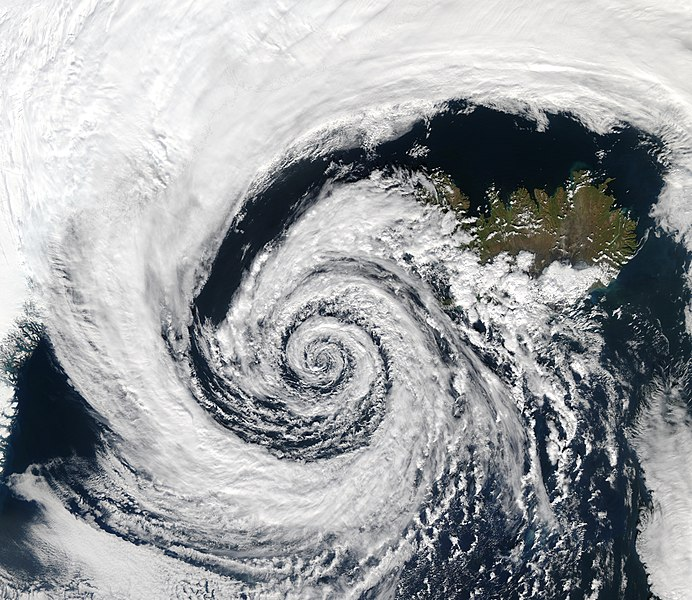
\includegraphics[width=0.6\textwidth]{images/cyclone.jpg}
      \caption{Cyclone on the atmosphere (large-scale). \cite{wikimedia_commons}}
    \end{figure}
  \end{minipage}\hfill
  \begin{minipage}{0.49\textwidth}
    \begin{figure}
      \centering
      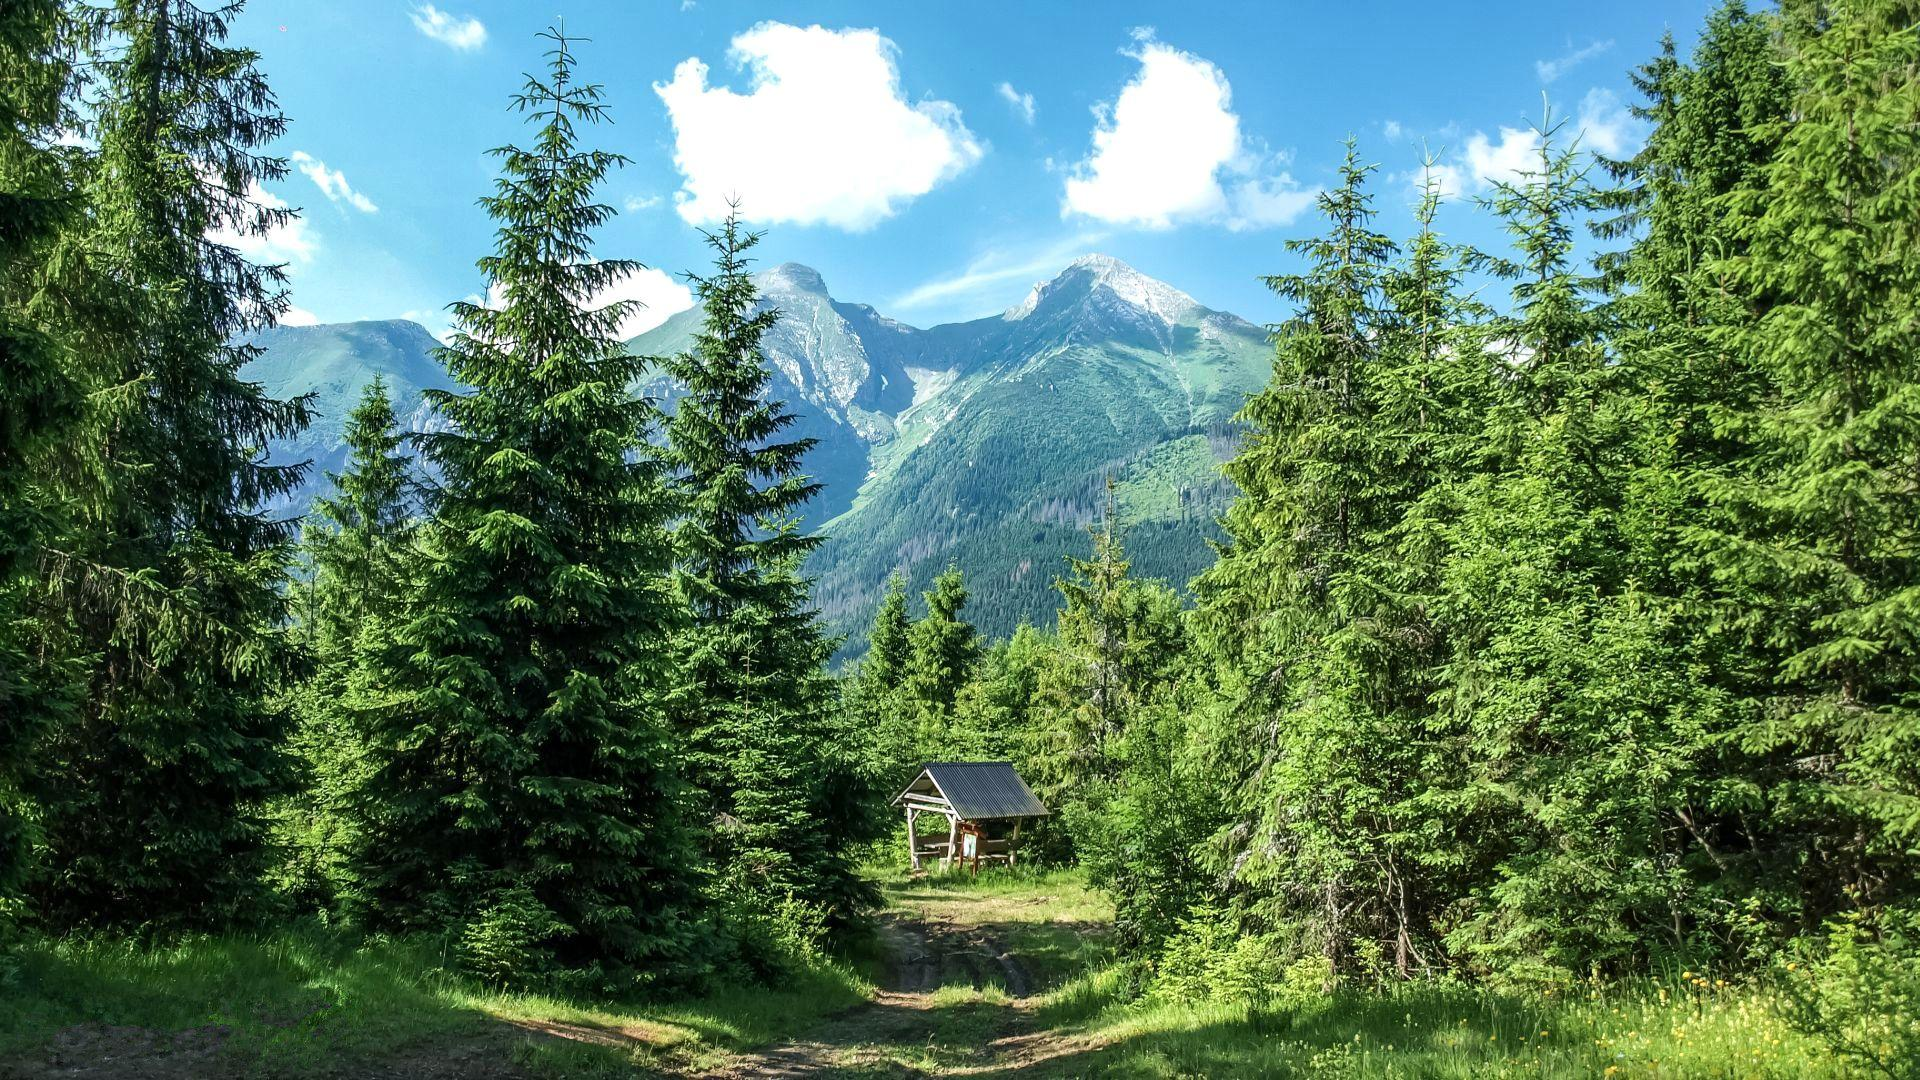
\includegraphics[width=0.8\textwidth]{images/tree.jpg}
      \caption{Leaves on the trees of the surface of the Earth (small-scale). \cite{tree}}
    \end{figure}
  \end{minipage}
\end{frame}
\begin{frame}{Motivation}
  \begin{itemize}
    \item There have been many attempts to model these multiscale flows.
    \item One of the most popular methods are the so-called \textbf{toy-models}, which are simplified models that capture the main features of the flow and neglect the unimportant properties of the original system.
    \item Our approach is instead of simplifying the equations, we simplify the configuration space \cite{campolina}.
  \end{itemize}
\end{frame}
{
\setbeamercolor{background canvas}{bg=\mycolor}
\begin{frame}[plain]
  \centering\vfill\Huge
  Log-lattice model
  \vfill
\end{frame}
\addtocounter{framenumber}{-1}
}
\begin{frame}{Equations and lattice}
  Underlying equations:
  \begin{align*}
    \textbf{Physical space:}\qquad & \partial_t \vf{u} + (\vf{u}\cdot\nabla)\vf{u} = -\grad p + \nu\Delta\vf{u} + \vf{f}                                             \\
    \textbf{Fourier space:}\qquad  & \partial_t \widehat{u}_i + \ii k_j \widehat{u}_j * \widehat{u}_i = -\ii k_i \widehat{p} - \nu k^2 \widehat{u}_i + \widehat{f}_i \\
                                   & (k^2 = k_1^2 + k_2^2 + k_3^2)
  \end{align*}

  \begin{minipage}{0.39\textwidth}
    Lattice (in each dimension):
    $$\Lambda:=\{\pm \lambda^n\}_{n\in\mathbb{Z}}\cup\{0\}$$
  \end{minipage}\hfill
  \begin{minipage}{0.59\textwidth}
    \begin{figure}
      \centering
      \includegraphics[width=0.9\textwidth]{images/lattice.pdf}
      \caption{Logarithmic lattices}
    \end{figure}
  \end{minipage}
\end{frame}
\begin{frame}{Choices for $\lambda$}
  We need to ensure that all the operations can be properly defined on the lattice. The main constraints are due to the convolution:
  \begin{equation}\label{eq:convolution}
    (f*g)(k) = \sum_{\substack{p,q\in \Lambda\\p+q=k}} f(p)g(q)
  \end{equation}
  We want to find $\lambda>0$ such that the sum of \eqref{eq:convolution} is non-trivial. For this we need to find the set of $\lambda$ such that the equation
  \begin{equation}
    \pm\lambda^a  \pm\lambda^b = \pm\lambda^c
  \end{equation}
  has non-trivial integer solutions $(a,b,c)\in\ZZ^3$.
  Some solutions are:
  \begin{align*}
    \lambda                            & = 2                    \qquad\quad\! (\text{5 terms in the sum}) \\
    \text{Golden ratio:}\qquad \varphi & \approx 1.618\quad (\text{8 terms in the sum})                   \\
    \text{plastic number:}\qquad\sigma & \approx 1.325\quad (\text{14 terms in the sum})
  \end{align*}
\end{frame}
\begin{frame}{Preservation of properties}
  Some preserved symmetry groups \cite{campolina}:
  \begin{itemize}
    \item Time and space translations.
    \item Scale invariance: $\widehat{\vf{u}}(\vf{k},t) \rightsquigarrow \lambda^h \widehat{\vf{u}}(\lambda^n \vf{k},\lambda^(h-n) t)$, $\forall h\in \RR, n\in\ZZ$ and $\lambda$ the lattice parameter.
    \item Isotropy and parity: $\widehat{\vf{u}}(\vf{k},t) \rightsquigarrow \vf{R}^{-1} \widehat{\vf{u}}(\vf{R}\vf{k},t)$, where $\vf{R}$ is any element of the group of cube symmetries.
  \end{itemize}
  Energy $\mathcal{E}=\frac{1}{2} \langle {\vf{u}}, {\vf{u}} \rangle$ and helicity $\mathcal{H}=\langle {\vf{u}}, {\vf{\omega}} \rangle$ are also preserved.

  % The inner product on the lattice is defined as:
  % \begin{align*}
  %   \langle f, g \rangle           & = \sum_{\vf{k}\in\Lambda^3} f(\vf{k})\overline{g(\vf{k})}                        \\
  %   \langle \vf{f}, \vf{g} \rangle & = \langle f_1, g_1 \rangle + \langle f_2, g_2 \rangle + \langle f_3, g_3 \rangle
  % \end{align*}
\end{frame}
{
\setbeamercolor{background canvas}{bg=\mycolor}
\begin{frame}[plain]
  \centering\vfill\Huge
  Results
  \vfill
\end{frame}
\addtocounter{framenumber}{-1}
}
\begin{frame}{Blow up in incompressible 3D Euler equations}
  \begin{itemize}
    \item Comparison between lattices with $\lambda=\varphi$ and $\lambda=\sigma$.
    \item Characterization of the blow up: $\omega_\text{max}:=\max_{\vf{k}} |\widehat{\vf{\omega}}(\vf{k},t)|\to \infty$.
    \item $\omega_\text{max}\sim (t_b - t)^{-1}$, where $t_b$ is the blow up time.
    \item The blow up travels at constant average speed $\gamma \approx 2.70$.
    \item $E(k) \sim k^{-\xi}$, $\xi =3-2/\gamma\approx 2.26$.
  \end{itemize}
  \begin{minipage}{0.49\textwidth}
    \begin{figure}
      \centering
      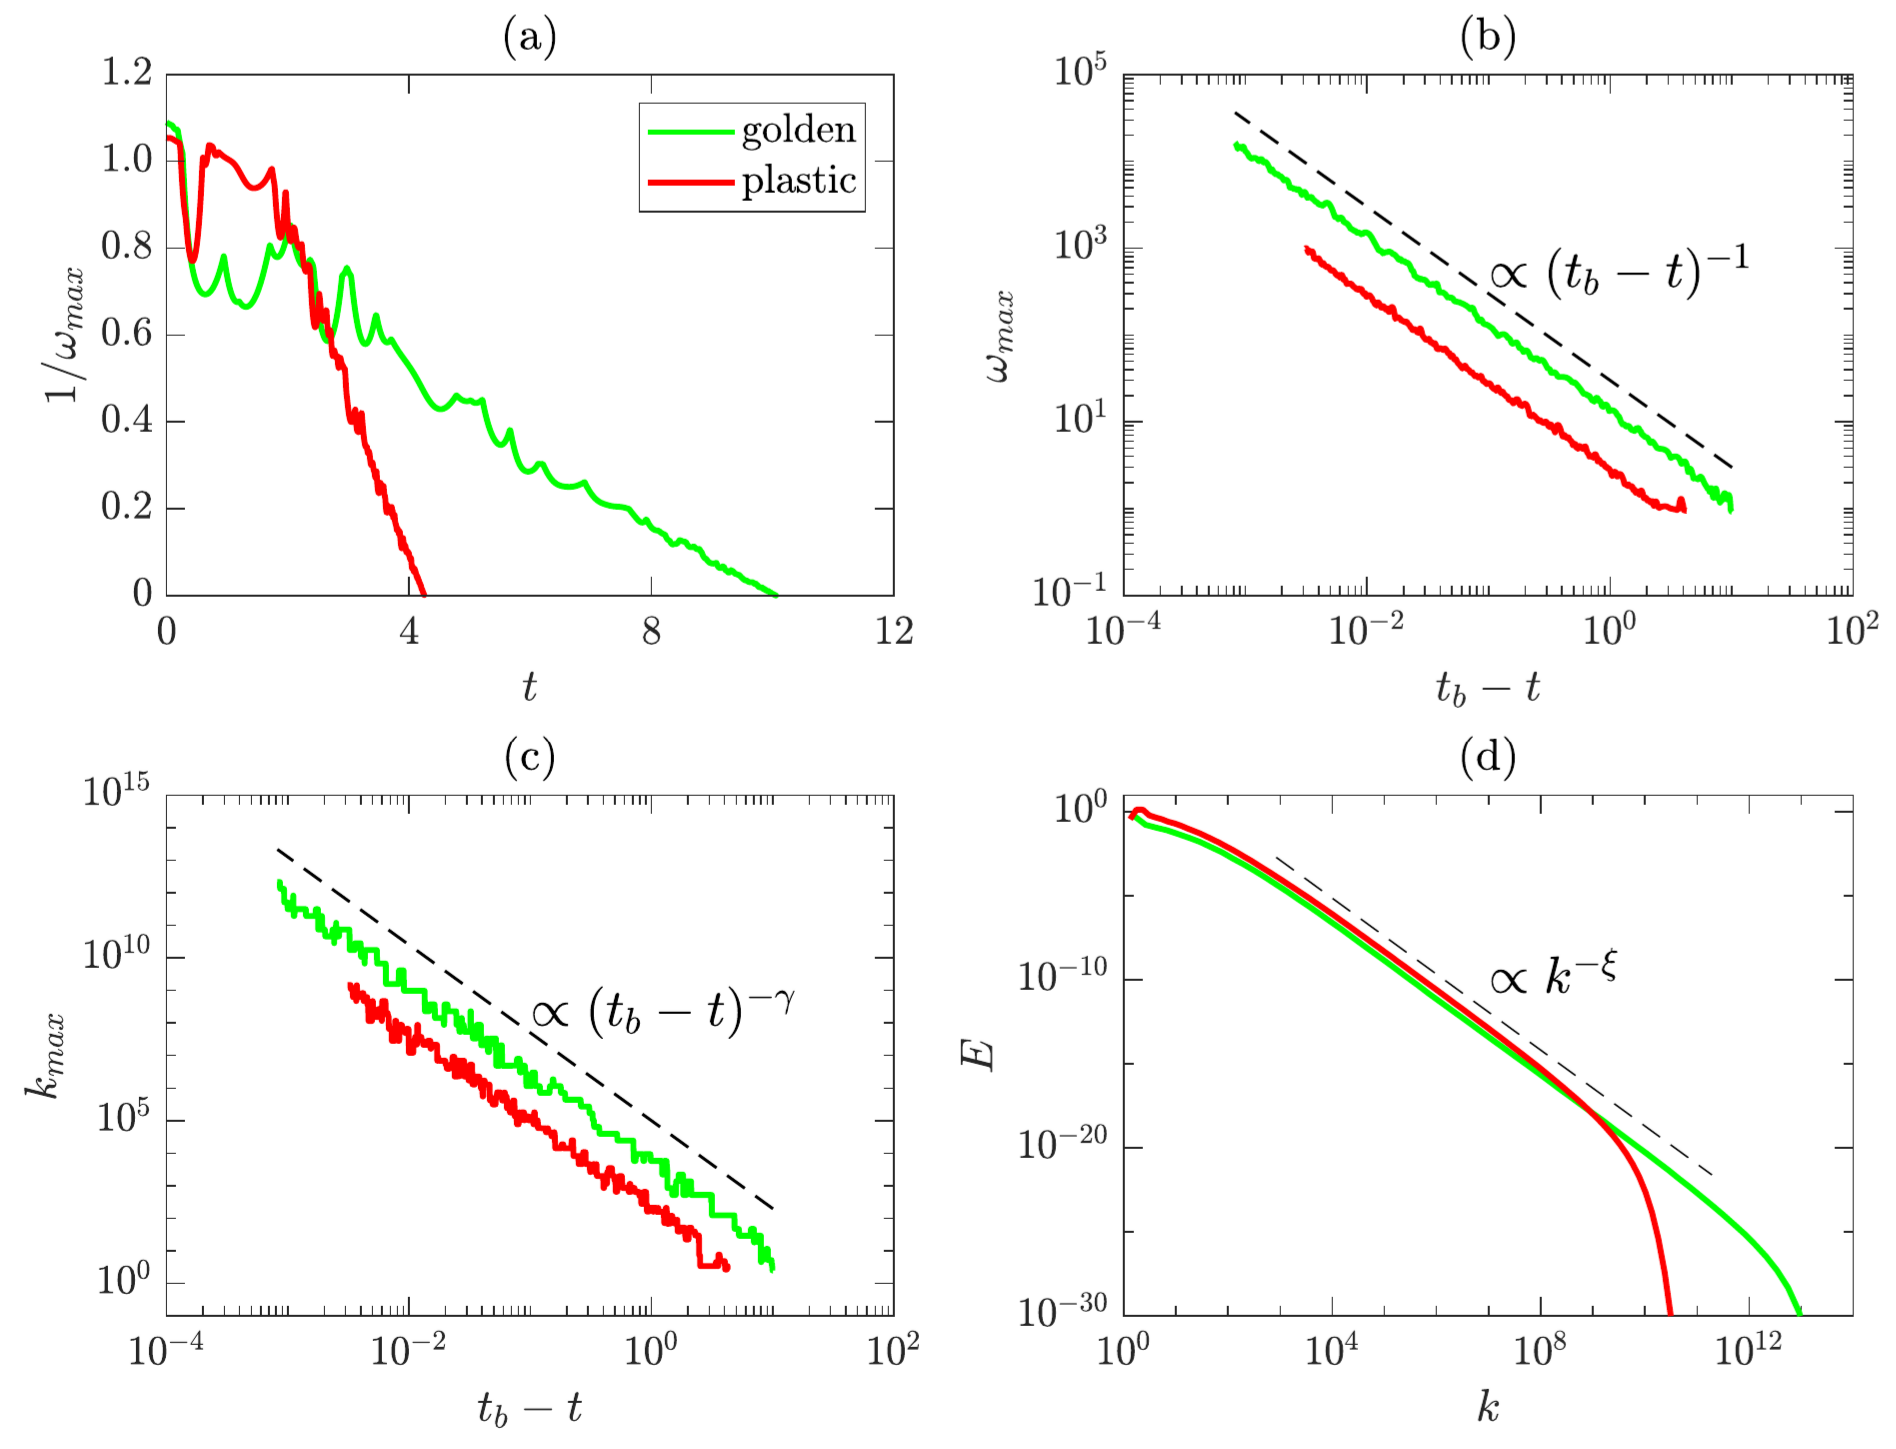
\includegraphics[width=0.8\textwidth]{images/blowup-1.png}
      \caption{Evolution of $\omega_\text{max}$, $k_\text{max}$ and $E(k)$. \cite{campolina}}
    \end{figure}
  \end{minipage}\hfill
  \begin{minipage}{0.49\textwidth}
    \begin{figure}
      \centering
      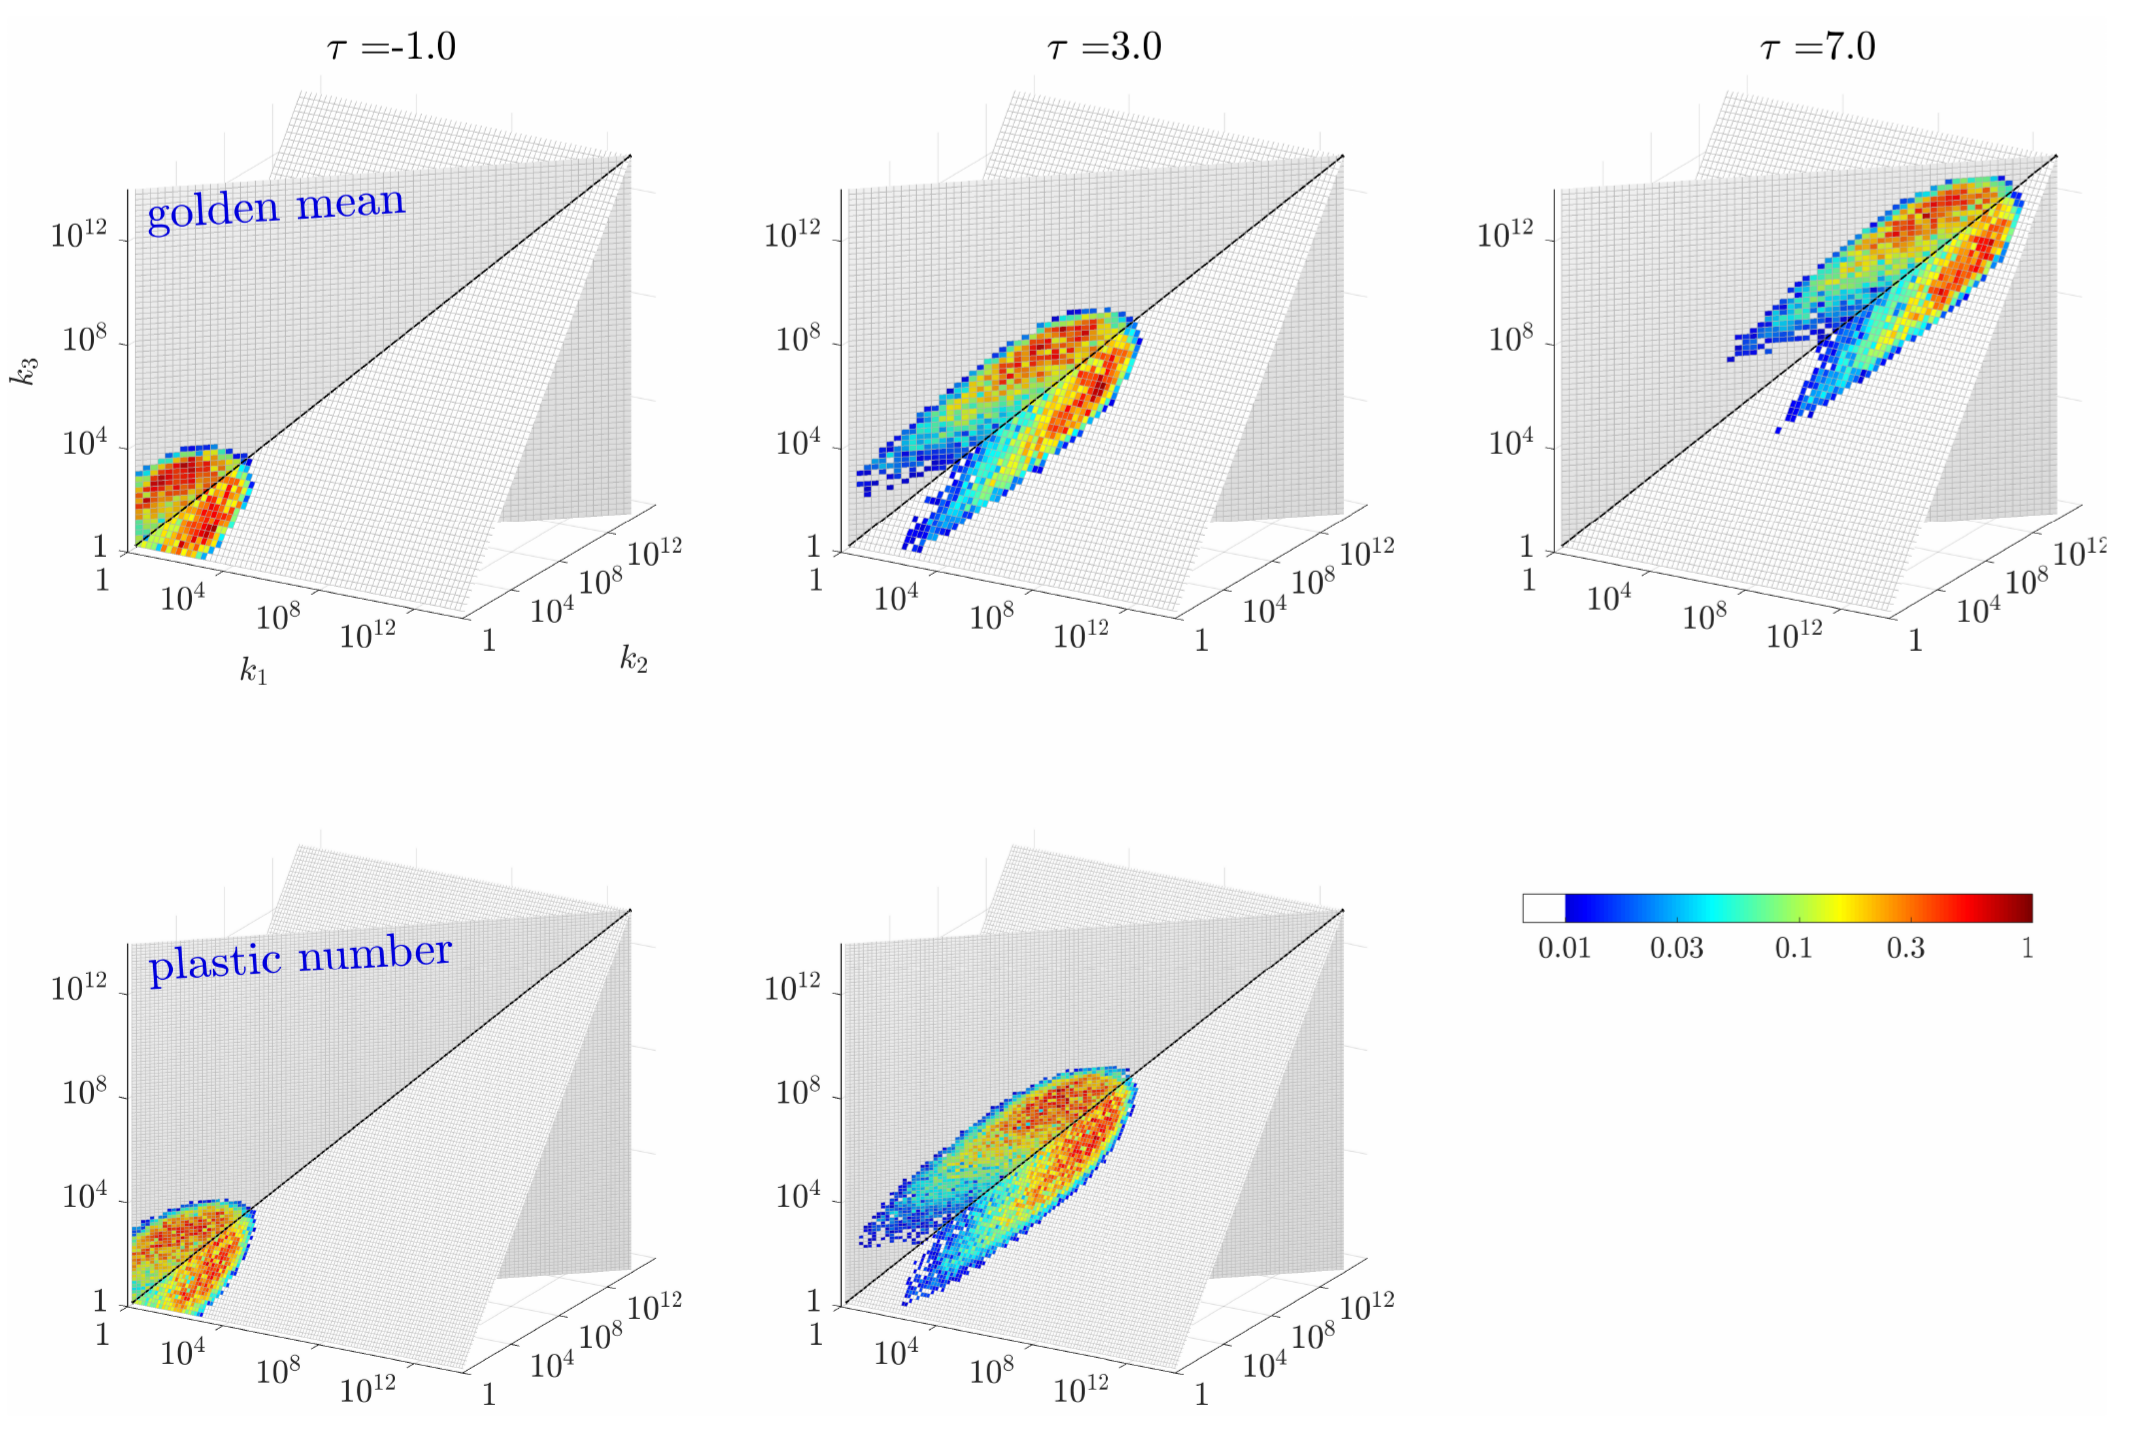
\includegraphics[width=0.9\textwidth]{images/blowup-2.png}
      \caption{Renormalized vorticities in Fourier space. \cite{campolina}}
    \end{figure}
  \end{minipage}
  \vspace{-0.5cm}
\end{frame}
\begin{frame}{Viscous incompressible flow and turbulence}
  \begin{minipage}{0.39\textwidth}
    \textbf{Dissipation anomaly:}
    $$
      \partial_t E_k + \Pi_k = -\epsilon_k + I_k
    $$
    \begin{figure}
      \centering
      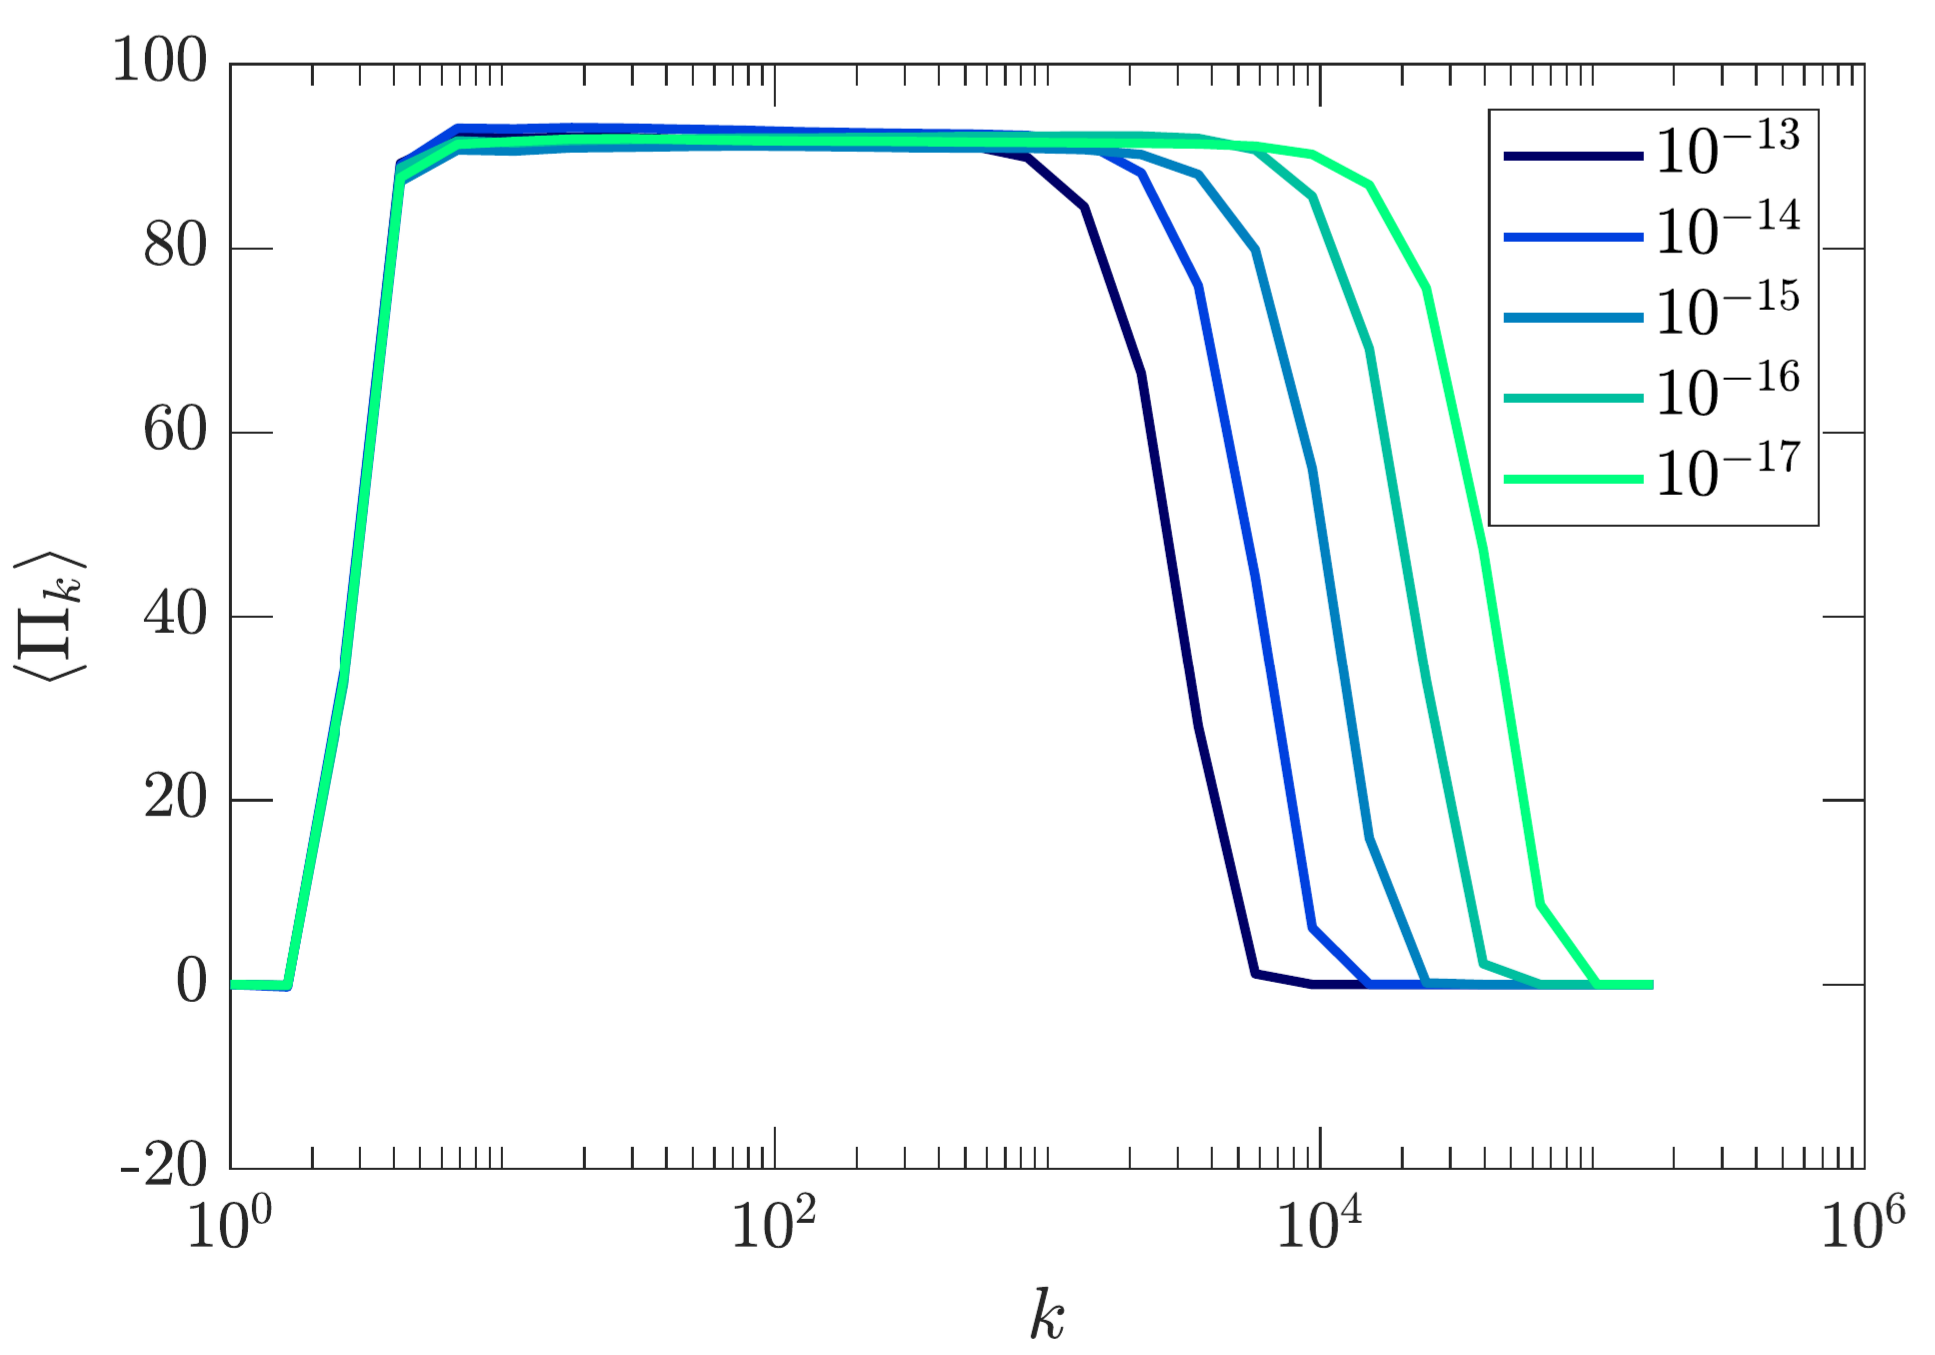
\includegraphics[width=0.9\textwidth]{images/viscous-1.png}
      \caption{Mean flux $\langle \Pi_k\rangle$ for different viscosities $\nu$. \cite{campolina}}
    \end{figure}
  \end{minipage}\hfill
  \begin{minipage}{0.59\textwidth}
    \textbf{Statistics of Fourier modes:}
    \begin{itemize}
      \item In the inertial range, the PDFs of the real part of the velocity behave as Gaussian.
      \item In the viscous range, the PDFs display some intermittency.
    \end{itemize}
    \begin{figure}
      \centering
      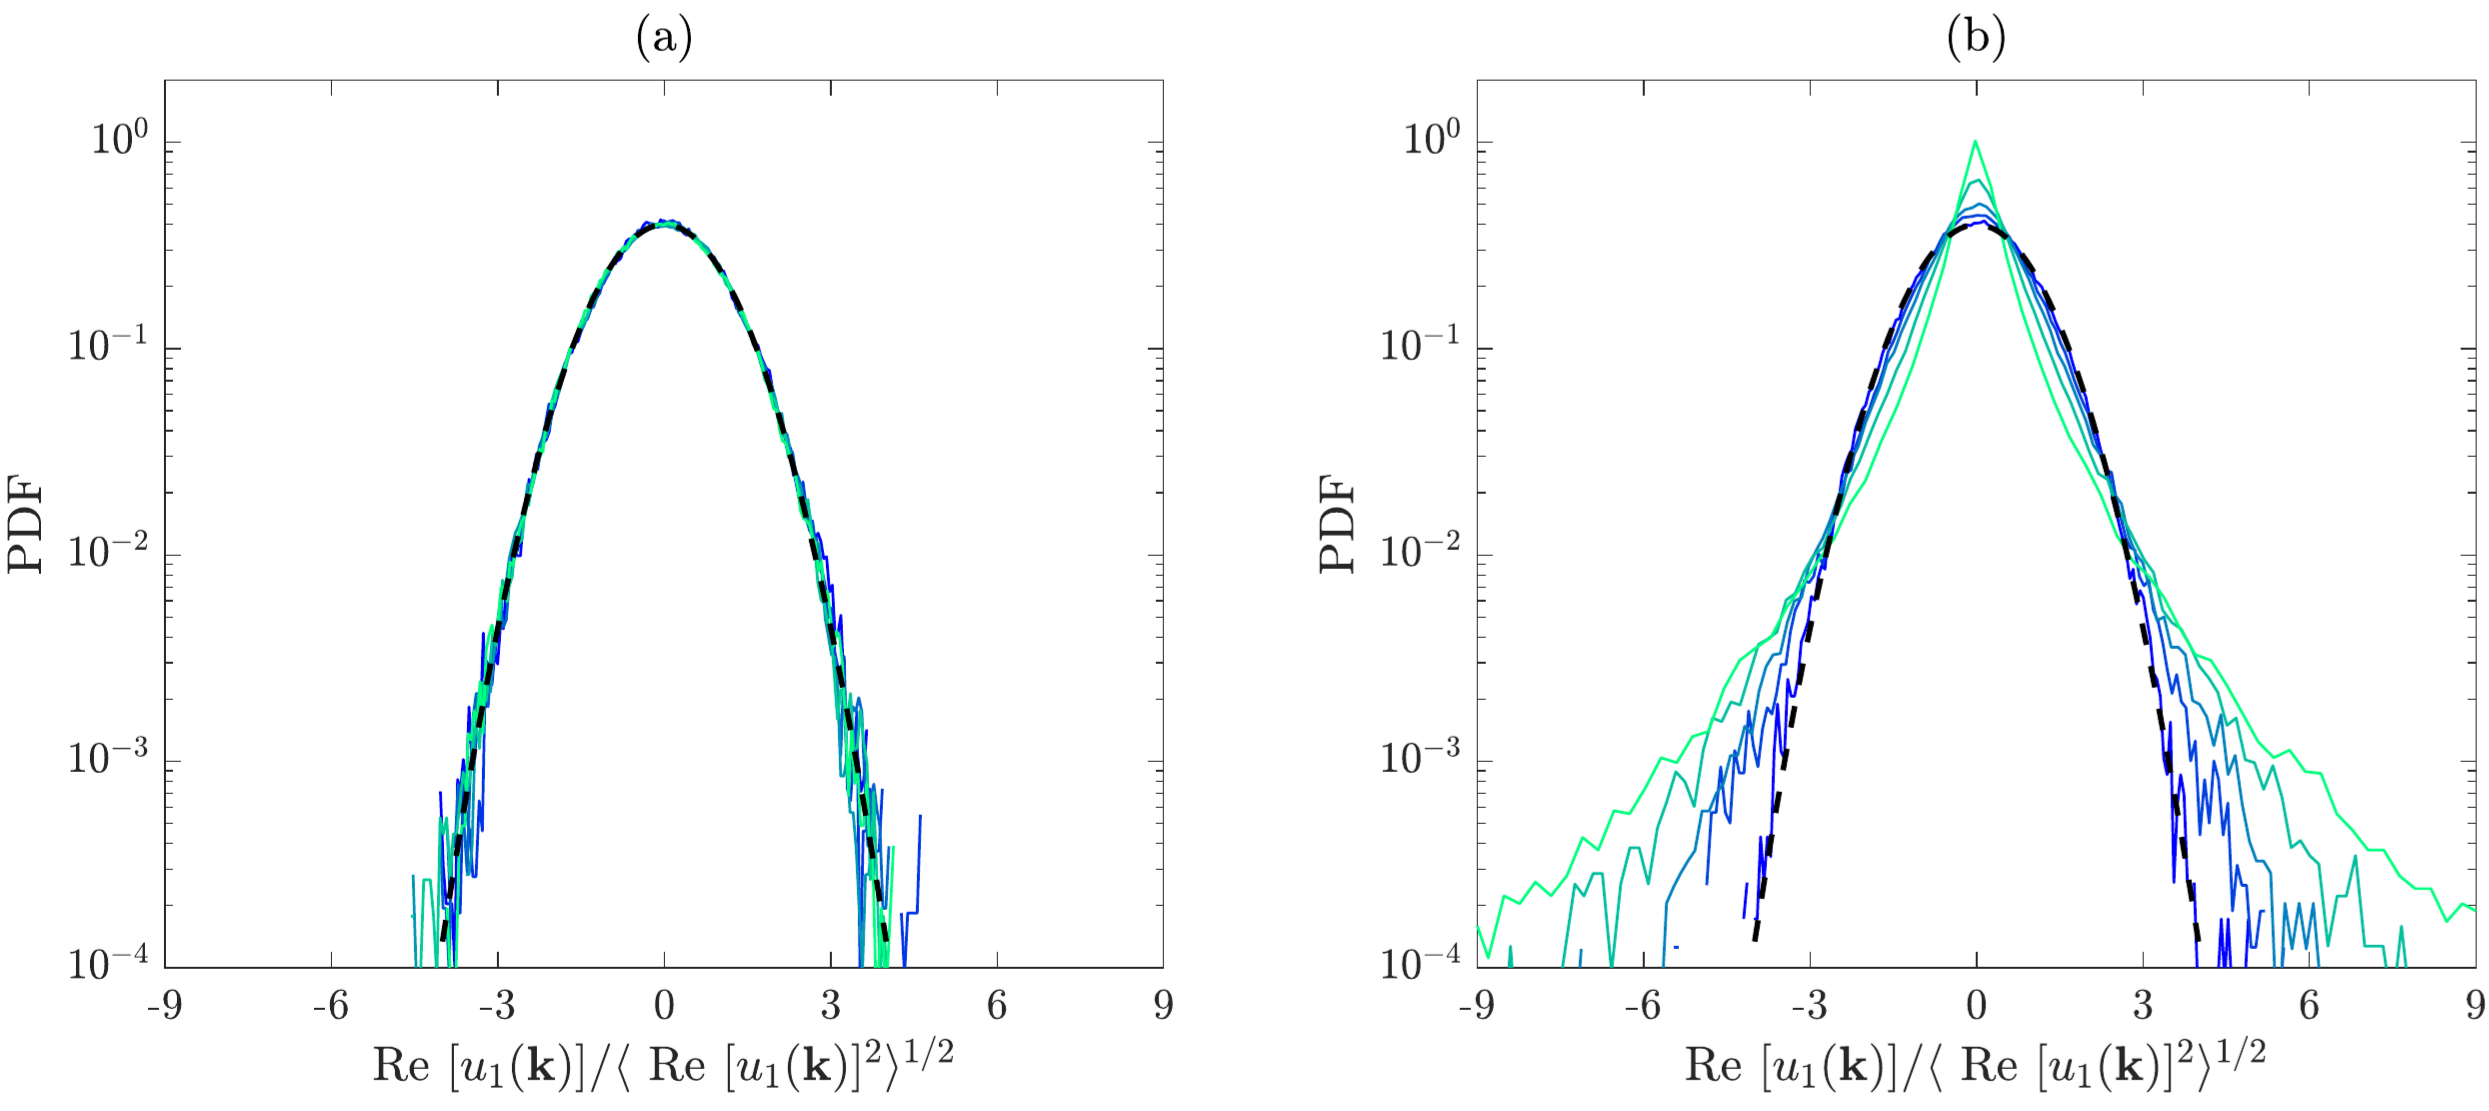
\includegraphics[width=\textwidth]{images/viscous-2.png}
      \caption{Normalized PDFs of the real part of x velocity. (a) Statistics of inertia-range wave vectors $\vf{k}_n:=\lambda^n(1,1,1)$, $n=10,...,15$. (b) Statistics of viscous-range wave vectors $\vf{k}_n$, $n=18,...,22$. \cite{campolina}}
    \end{figure}
  \end{minipage}
\end{frame}
{
\setbeamercolor{background canvas}{bg=\mycolor}
\begin{frame}[plain]
  \centering\vfill\Huge
  Conclusions
  \vfill
\end{frame}
\addtocounter{framenumber}{-1}
}
\begin{frame}{Conclusions}
  \textbf{Advantages of using logarithmic lattices:}
  \begin{itemize}
    \item Huge reduction in the number of active modes. For $\lambda=\varphi$, we go from $N\sim 10^{33}$ to $N\sim 160$.
    \item Most of the symmetries and conservation laws of the original system are preserved.
  \end{itemize}
  \textbf{Disadvantages:}
  \begin{itemize}
    \item Unable to describe \textbf{non-local} interactions.
    \item Cannot capture the \textbf{dispersive} properties of some systems.

          If $\widehat{u}\simeq \widehat{u}_0 e^{\ii (kx + \omega t)}$ and $\omega = k^\alpha$, then the interactions between waves with different $\omega$ are not well described (for $\alpha\neq 1$).
  \end{itemize}
\end{frame}
\begin{frame}[noframenumbering]{References}
  \printbibliography[heading=none]
\end{frame}
\end{document}